\documentclass[twoside]{article}

%\usepackage{aistats2021}
% If your paper is accepted, change the options for the package
% aistats2021 as follows:
%
\usepackage[accepted]{aistats2021}
\usepackage{amsfonts}
\usepackage{graphicx}
%
% This option will print headings for the title of your paper and
% headings for the authors names, plus a copyright note at the end of
% the first column of the first page.

% If you set papersize explicitly, activate the following three lines:
%\special{papersize = 8.5in, 11in}
%\setlength{\pdfpageheight}{11in}
%\setlength{\pdfpagewidth}{8.5in}

% If you use natbib package, activate the following three lines:
%\usepackage[round]{natbib}
%\renewcommand{\bibname}{References}
%\renewcommand{\bibsection}{\subsubsection*{\bibname}}

% If you use BibTeX in apalike style, activate the following line:
%\bibliographystyle{apalike}

\begin{document}

% If your paper is accepted and the title of your paper is very long,
% the style will print as headings an error message. Use the following
% command to supply a shorter title of your paper so that it can be
% used as headings.
%
%\runningtitle{I use this title instead because the last one was very long}

% If your paper is accepted and the number of authors is large, the
% style will print as headings an error message. Use the following
% command to supply a shorter version of the authors names so that
% they can be used as headings (for example, use only the surnames)
%
%\runningauthor{Surname 1, Surname 2, Surname 3, ...., Surname n}

\twocolumn[

\aistatstitle{TDHNN: Time-Dependent Hamiltonian Neural Networks }

\aistatsauthor{ Shaan A. Desai$^{1,2}$ \And David Sondak$^{2}$ \And  Marios Mathiakis$^{2}$ }

\aistatsaddress{ Machine Learning Research Group \\University of Oxford $^1$ \And Institute of Applied Computational Science \\ Harvard University $^2$ } ]



\begin{abstract}

Deep networks embedded with physically-informed priors demonstrate  remarkable performance in accurately learning and predicting non-linear dynamical systems. In particular, energy-conserving networks designed to exploit the Hamiltonian formalism show strong and consistent performance in learning autonomous systems that depend implicitly on time. Here, we extend this work to include an explicit time-dependence that generalizes the learning to include non-autonomous dynamical systems. We achieve this generalisation by embedding the port-Hamiltonian formalism into our neural network. We show that such a system can learn complex forced and damped dynamics, including the chaotic duffing equation, as well as maintain strong performance in settings that have no explicit time-dependence.

%Unlike vanilla Artificial Neural Networks, Neural Networks embedded with physically-informed priors achieve remarkable results in accurately learning and predicting non-linear dynamical systems.
% despite this success, their generalization is often limited by the available training data which in practice only consists of a few short-range trajectories. naturally we might ask how we can generalize to unseen timesteps better?
% Despite this success, their generalization performance is often limited to short-range trajectories that run for less than the final training time. The performance degradation is due to state and energy drift induced by errors accumulating over time and it poses a critical challenge to learning highly non-linear and chaotic long-range dynamics precisely when data for only a limited number of short-range trajectories are available. One proposed solution to this challenge has been to incorporate symplectic integrators that aim to preserve the symplectic flow. Here, we present an alternative, an L1 penalty of the Hamiltonian derivative with respect to time: $d\mathcal{H}(p,q,t)/dt$. The inclusion of this term, a straightforward addition to the network, enforces the Hamiltonian to remain constant in time for a given trajectory. We empirically illustrate the stabilising effect this penalty has on our network. In addition, we use it solve problems in non-linear dynamics such as heinon-heiles, 3-body problem and double pendulum.
\end{abstract}

\begin{figure}[h!]
\centering
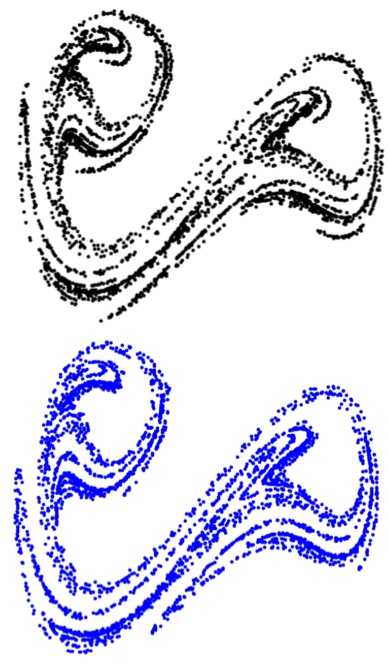
\includegraphics[width=0.4\textwidth, height=9cm]{figures/Picture1.png}
\caption{Poincar\'e Section of a duffing oscillator in a chaotic regime. Top is the ground truth and bottom is the predicted. Predictions are made using TDHNN which is trained on 2000 points.}
\end{figure}
\section{Introduction}

Neural networks, as universal function approximators, have shown resounding success across a host of domains. However, their performance in learning physical systems has often been limited. New research aimed at \textit{scientific machine learning} - a branch that tackles scientific problems with domain-specific ML, is paving a way to address these challenges. It has been shown that prior theoretical information embedded in networks, such as Hamiltonian mechanics \cite{greydanus} demonstrate a significant performance uplift in learning. This excitement has spurred others to work with Lagrangians, ODEs and even graphs in order to tackle the learning of dynamical systems. Despite their widespread adoption, a major bottleneck of many of the existing methods is the lack of an explicit-time dependence as is evident across a host of forced dynamical systems. The most general form of Hamilton's equations, includes an explicit time dependence term. We show that the addition of this term, coupled with a few intuitive regularizations can induce networks to learn from both autonomous and non-autonomous settings. We extensively benchmark this addition across multiple datasets and consistently find the inclusion to be of benefit. Furthermore, we emphasise that the constraint is an easy plug-and-play addition to existing networks and illustrate how existing networks such as HNN, Symp ODEN and Hnets benefit from its inclusion. 

\section{Background}

\subsection{Hamiltonian Neural Networks}

Recently, \cite{greydanus_hamiltonian_2019} demonstrated that dynamic predictions through time can be improved using Hamiltonian Neural Networks (HNNs) which endow models with a Hamiltonian constraint. The Hamiltonian is an important representation of a dynamical system because it is one of two well-known approaches that generalizes classical mechanics. The Hamiltonian $\mathcal{H}$ is a scalar function of position $\mathbf{q} = (q_1,q_2,....,q_M)$ and momentum $\mathbf{p} = (p_1,p_2,....,p_M)$. It is a powerful representation because it allows us to obtain the time derivatives of the inputs $(\dot{q},\dot{p})$ by simply differentiating the Hamiltonian with respect to its inputs (see Eqn. \ref{eqn.hamiltonian}.)
\begin{equation}
\frac{\mathrm{d}\mathbf{q}}{\mathrm{d}t} = \frac{\partial \mathcal{H}}{\partial \mathbf{p}}, ~~~
\frac{\mathrm{d}\mathbf{p}}{\mathrm{d}t} = -\frac{\partial \mathcal{H}}{\partial \mathbf{q}}
\label{eqn.hamiltonian}
\end{equation}
As a consequence, it is noted in \cite{greydanus_hamiltonian_2019} that by parametrizing the Hamiltonian with a neural network e.g. $H_{\theta}(\mathbf{q},\mathbf{p})$ where $\theta$ represents a deep neural network, one can easily obtain the system's dynamics by differentiating (via autograd) the Hamiltonian with its inputs. This information allows us to build two 1st-order differential equations which can be used to update the state space, $(\mathbf{q},\mathbf{p})$. Equation \ref{eqn.action_int} shows this integral, in which we define the symplectic gradient $\mathbf{S}  = \left [ \frac{\partial \mathcal{H}}{\partial \mathbf{p}},-\frac{\partial \mathcal{H}}{\partial \mathbf{q}} \right ] $:
\begin{equation}
(\mathbf{q},\mathbf{p})_{t+1} = (\mathbf{q},\mathbf{p})_t + \int_t^{t+1} \mathbf{S}(\mathbf{q},\mathbf{p}) \mathrm{d}t
\label{eqn.action_int}
\end{equation}
However, this is not the only benefit in learning a Hamiltonian. Another key attribute of the Hamiltonian is that the vector field $\mathbf{S}$ is a symplectic gradient meaning $\mathcal{H}$ remains constant as long as state vectors are integrated along $\mathbf{S}$. This result links the Hamiltonian with the total energy of the system such that $\mathcal{H}(\mathbf{q},\mathbf{p}) = E_{tot}$ for many physical systems. Therefore, the Hamiltonian is a powerful inductive bias that can be utilised to evolve a physical state while maintaining energy conservation. 

Although this formalism is compact and powerful, it does not readily generalize to damped or forced system. As such, we refer to port-Hamiltonian systems.

\subsection{Port-Hamiltonians}

Port-Hamiltonians are a formalism that allow us to incorporate damping and forcing terms. One formalism outlined in \cite{dissipative sympoden} shows how to represent a general form for such a system. We extend that work to include time-dependent forcing and eliminate the need for an explicit control input $u$. This results in the following equation:

\begin{equation}
\begin{bmatrix}
\dot{\mathbf{q}} \\
\dot{\mathbf{p}}
\end{bmatrix}
=
\Bigg(\begin{bmatrix}
0 & \mathbf{I} \\
-\mathbf{I} & 0
\end{bmatrix} +
\begin{bmatrix}
0 & 0 \\
0 & \mathbf{D}_{\theta_2}(\mathbf{q})
\end{bmatrix}
 \Bigg)
 \begin{bmatrix}
\frac{\partial \mathcal{H}_{\theta_1}}{\partial \mathbf{q}} \\
\frac{\partial \mathcal{H}_{\theta_1}}{\partial \mathbf{p}}
\end{bmatrix}
+
\begin{bmatrix}
0 \\
\mathbf{g}(\mathbf{q})
\end{bmatrix}
F_{\theta_3}(t)
\end{equation}

where $\mathbf{D}_{\theta_2}(q)$ is the damping term and $g(q)F_{\theta_3}(t)$ is the forcing term. 

Given this general formalism, we make some simplifications. Here, instead of using a generalized semi-positive definite damping matrix, we simply aim at learning the lower right term which is most often independent of $\mathbf{q}$. As such, we parametrize $\mathbf{D}$ with a single, scalar learnable parameter. Secondly, for many physical systems, $g(q)$ is also a scalar quantity, so we abstract this scalar learning into $F(t)$ by setting $g(q) = 1$.
 

\section{Method}

\begin{equation}
Loss =\left\| \frac{\partial \mathcal{H}_{\theta_1}}{\partial \mathbf{q}} +  \frac{\partial \mathbf{p}}{\partial t} \right\| +\left\| \frac{\partial \mathcal{H}_{\theta_1}}{\partial \mathbf{p}} -  \frac{\partial \mathbf{q}}{\partial t} \right\|+ \alpha_{reg}| F_{\theta_3} (t)| + \beta_{reg}|D_{\theta_2}| 
\end{equation}

To learn the dynamics, we feed in a state-vector $S_t = [\mathbf{q},\mathbf{p},\mathbf{t}]$. The first neural-network consists of 3 hidden layers designed to predict $H$ from $[q,p]$ data. The second neural-network consists of a single weight parameter designed to learn the damping coefficient $D$ and the third neural-network consists of 2 hidden layers designed to predict $F(t)$ from t. We use an L2-norm penalty for the predicted state-vectors and an L1-norm for force and damping to encourage sparsity. We do this because we would like our networks to identify classical autonomous systems (which may not have force or time) as well as non-autonomous systems. For our experiments we use 200 hidden layers and find that most activations such as tanh, sin and cos yield comparable results. To benchmark our method, as \cite{greydanus} do, we use a baseline NN that takes in $S_t$ and predicts $[\dot{q},\dot{p}]$. We also take the straightforward extension of HNN to include time as a variable input.



\section{FIRST LEVEL HEADINGS}

First level headings are all caps, flush left, bold, and in point size
12. Use one line space before the first level heading and one-half line space
after the first level heading.

\subsection{Second Level Heading}

Second level headings are initial caps, flush left, bold, and in point
size 10. Use one line space before the second level heading and one-half line
space after the second level heading.

\subsubsection{Third Level Heading}

Third level headings are flush left, initial caps, bold, and in point
size 10. Use one line space before the third level heading and one-half line
space after the third level heading.

\paragraph{Fourth Level Heading}

Fourth level headings must be flush left, initial caps, bold, and
Roman type.  Use one line space before the fourth level heading, and
place the section text immediately after the heading with no line
break, but an 11 point horizontal space.

%%%
\subsection{Citations, Figure, References}


\subsubsection{Citations in Text}

Citations within the text should include the author's last name and
year, e.g., (Cheesman, 1985). 
%Apart from including the author's last name and year, citations can follow any style, as long as the style is consistent throughout the paper.  
Be sure that the sentence reads
correctly if the citation is deleted: e.g., instead of ``As described
by (Cheesman, 1985), we first frobulate the widgets,'' write ``As
described by Cheesman (1985), we first frobulate the widgets.''


The references listed at the end of the paper can follow any style as long as it is used consistently.

%Be sure to avoid
%accidentally disclosing author identities through citations.

\subsubsection{Footnotes}

Indicate footnotes with a number\footnote{Sample of the first
  footnote.} in the text. Use 8 point type for footnotes. Place the
footnotes at the bottom of the column in which their markers appear,
continuing to the next column if required. Precede the footnote
section of a column with a 0.5 point horizontal rule 1~inch (6~picas)
long.\footnote{Sample of the second footnote.}

\subsubsection{Figures}

All artwork must be centered, neat, clean, and legible.  All lines
should be very dark for purposes of reproduction, and art work should
not be hand-drawn.  Figures may appear at the top of a column, at the
top of a page spanning multiple columns, inline within a column, or
with text wrapped around them, but the figure number and caption
always appear immediately below the figure.  Leave 2 line spaces
between the figure and the caption. The figure caption is initial caps
and each figure should be numbered consecutively.

Make sure that the figure caption does not get separated from the
figure. Leave extra white space at the bottom of the page rather than
splitting the figure and figure caption.
\begin{figure}[h]
\vspace{.3in}
\centerline{\fbox{This figure intentionally left non-blank}}
\vspace{.3in}
\caption{Sample Figure Caption}
\end{figure}

\subsubsection{Tables}

All tables must be centered, neat, clean, and legible. Do not use hand-drawn tables.
Table number and title always appear above the table.
See Table~\ref{sample-table}.

Use one line space before the table title, one line space after the table title,
and one line space after the table. The table title must be
initial caps and each table numbered consecutively.

\begin{table}[h]
\caption{Sample Table Title} \label{sample-table}
\begin{center}
\begin{tabular}{ll}
\textbf{PART}  &\textbf{DESCRIPTION} \\
\hline \\
Dendrite         &Input terminal \\
Axon             &Output terminal \\
Soma             &Cell body (contains cell nucleus) \\
\end{tabular}
\end{center}
\end{table}

\section{SUPPLEMENTARY MATERIAL}

If you need to include additional appendices during submission, you can include them in the supplementary material file.
You can submit a single file of additional supplementary material which may be either a pdf file (such as proof details) or a zip file for other formats/more files (such as code or videos). 
Note that reviewers are under no obligation to examine your supplementary material. 
If you have only one supplementary pdf file, please upload it as is; otherwise gather everything to the single zip file.

You must use \texttt{aistats2021.sty} as a style file for your supplementary pdf file and follow the same formatting instructions as in the main paper. 
The only difference is that it must be in a \emph{single-column} format.
You can use \texttt{supplement.tex} in our starter pack as a starting point.
Alternatively, you may append the supplementary content to the main paper and split the final PDF into two separate files.

\section{SUBMISSION INSTRUCTIONS}

To submit your paper to AISTATS 2021, please follow these instructions.

\begin{enumerate}
    \item Download \texttt{aistats2021.sty}, \texttt{fancyhdr.sty}, and \texttt{sample\_paper.tex} provided in our starter pack. 
    Please, do not modify the style files as this might result in a formatting violation.
    
    \item Use \texttt{sample\_paper.tex} as a starting point.
    \item Begin your document with
    \begin{flushleft}
    \texttt{\textbackslash documentclass[twoside]\{article\}}\\
    \texttt{\textbackslash usepackage\{aistats2021\}}
    \end{flushleft}
    The \texttt{twoside} option for the class article allows the
    package \texttt{fancyhdr.sty} to include headings for even and odd
    numbered pages.
    \item When you are ready to submit the manuscript, compile the latex file to obtain the pdf file.
    \item Check that the content of your submission, \emph{excluding} references, is limited to \textbf{8 pages}. The number of pages containing references alone is not limited.
    \item Upload the PDF file along with other supplementary material files to the CMT website.
\end{enumerate}

\subsection{Camera-ready Papers}

%For the camera-ready paper, if you are using \LaTeX, please make sure
%that you follow these instructions.  
% (If you are not using \LaTeX,
%please make sure to achieve the same effect using your chosen
%typesetting package.)

If your papers are accepted, you will need to submit the camera-ready version. Please make sure that you follow these instructions:
\begin{enumerate}
    %\item Download \texttt{fancyhdr.sty} -- the
    %\texttt{aistats2021.sty} file will make use of it.
    \item Change the beginning of your document to
    \begin{flushleft}
    \texttt{\textbackslash documentclass[twoside]\{article\}}\\
    \texttt{\textbackslash usepackage[accepted]\{aistats2021\}}
    \end{flushleft}
    The option \texttt{accepted} for the package
    \texttt{aistats2021.sty} will write a copyright notice at the end of
    the first column of the first page. This option will also print
    headings for the paper.  For the \emph{even} pages, the title of
    the paper will be used as heading and for \emph{odd} pages the
    author names will be used as heading.  If the title of the paper
    is too long or the number of authors is too large, the style will
    print a warning message as heading. If this happens additional
    commands can be used to place as headings shorter versions of the
    title and the author names. This is explained in the next point.
    \item  If you get warning messages as described above, then
    immediately after $\texttt{\textbackslash
    begin\{document\}}$, write
    \begin{flushleft}
    \texttt{\textbackslash runningtitle\{Provide here an alternative
    shorter version of the title of your paper\}}\\
    \texttt{\textbackslash runningauthor\{Provide here the surnames of
    the authors of your paper, all separated by commas\}}
    \end{flushleft}
    Note that the text that appears as argument in \texttt{\textbackslash
      runningtitle} will be printed as a heading in the \emph{even}
    pages. The text that appears as argument in \texttt{\textbackslash
      runningauthor} will be printed as a heading in the \emph{odd}
    pages.  If even the author surnames do not fit, it is acceptable
    to give a subset of author names followed by ``et al.''

    %\item Use the file sample\_paper.tex as an example.

    \item The camera-ready versions of the accepted papers are 8
      pages, plus any additional pages needed for references.

    \item If you need to include additional appendices,
      you can include them in the supplementary
      material file.

    \item Please, do not change the layout given by the above
      instructions and by the style file.

\end{enumerate}

\subsubsection*{Acknowledgements}
All acknowledgments go at the end of the paper, including thanks to reviewers who gave useful comments, to colleagues who contributed to the ideas, and to funding agencies and corporate sponsors that provided financial support. 
To preserve the anonymity, please include acknowledgments \emph{only} in the camera-ready papers.

\bibliography{references.bib}
\end{document}
